\chapter{METODE PENELITIAN}

Bab ini menjelaskan metode yang digunakan dalam penelitian secara rinci, meliputi rancangan penelitian, data dan sumber data, alat yang digunakan, serta tahapan sistematis dalam pengembangan sistem. Penelitian ini merupakan penelitian terapan dengan pendekatan rekayasa sistem yang berfokus pada perancangan dan implementasi sistem \textit{end-to-end} untuk \textit{Knowledge Graph Construction} (KGC) dan \textit{Hybrid Retrieval-Augmented Generation} (Hybrid Graph-RAG).

\subsection{Variabel Data dan Sumber Data}
\label{subsec:sumber-data}

Data yang dikumpulkan dalam penelitian ini merupakan data sekunder yang diperoleh dari basis data internal universitas dan pengindeks publikasi eksternal. Berbeda dengan penelitian survei yang menggunakan responden, penelitian ini menggunakan \textit{data records} yang merepresentasikan entitas akademik di lingkungan klaster Infokom UNESA.

Data yang digunakan mencakup empat sumber utama yang saling melengkapi untuk membentuk \textit{Academic Knowledge Graph}, sebagaimana dijabarkan pada Tabel~\ref{tab:deskripsi-dataset}.

\begin{table}[htbp]
    \centering
    \caption{Deskripsi Dataset dan Peran dalam Model Knowledge Graph}
    \label{tab:deskripsi-dataset}
    \renewcommand{\arraystretch}{1.5} % Memberi jarak antar baris agar rapi
    \begin{tabular}{|p{4.5cm}|p{5cm}|p{5.5cm}|}
        \hline
        \textbf{Nama Dataset} & \textbf{Definisi Operasional} & \textbf{Peran dalam Model (Entitas \& Relasi)} \\ 
        \hline
        \textbf{Data Profil Dosen} \newline (\texttt{dosen\_data.csv}) & 
        Data induk yang memuat identitas, afiliasi prodi, dan ID eksternal (Sinta, Scopus, Scholar) dari dosen klaster Infokom. & 
        Berperan sebagai \textit{Master Node} (\texttt{Researcher}). Menghubungkan seluruh entitas lain melalui ID unik. \\ 
        \hline
        \textbf{Data Publikasi Scopus} \newline (\texttt{scival\_filtered\_infokom.csv}) & 
        Metadata publikasi bereputasi tinggi yang memuat metrik kualitas seperti CiteScore dan Quartile. & 
        Membentuk node \texttt{Publication} dengan bobot kualitas tinggi. Digunakan untuk analisis sitasi dan performa riset. \\ 
        \hline
        \textbf{Data Riset Internal} \newline (\texttt{research.csv}) & 
        Rekam jejak proyek penelitian dan pengabdian yang didanai oleh universitas atau kementerian (SINTA). & 
        Membentuk node \texttt{Project} dan \texttt{Grant}. Memodelkan relasi kolaborasi internal (\texttt{COLLABORATES\_WITH}). \\ 
        \hline
        \textbf{Data Google Scholar} \newline (\texttt{publications\_scholar\_scraped.csv}) & 
        Kumpulan metadata publikasi luas beserta teks abstrak yang diambil menggunakan teknik \textit{scraping}. & 
        Sumber utama teks tidak terstruktur (\textit{unstructured text}) untuk proses \textit{embedding} vektor dan ekstraksi topik riset. \\ 
        \hline
    \end{tabular}
\end{table}

Keempat dataset tersebut kemudian diintegrasikan. Agar dapat diproses dalam \textit{pipeline} konstruksi graf, struktur atribut dari masing-masing dataset dideklarasikan tipe data dan fungsinya pada Tabel~\ref{tab:struktur-data}.

\begin{table}[htbp]
    \centering
    \caption{Struktur Atribut Data Utama}
    \label{tab:struktur-data}
    \renewcommand{\arraystretch}{1.3}
    \begin{tabular}{|l|l|l|p{5.5cm}|}
        \hline
        \textbf{Dataset} & \textbf{Nama Atribut} & \textbf{Tipe Data} & \textbf{Deskripsi} \\ 
        \hline
        \multirow{4}{*}{\textbf{Dosen}} 
        & \texttt{nidn} & String & Identitas unik nasional dosen. \\ 
        & \texttt{nama\_dosen} & String & Nama lengkap beserta gelar. \\ 
        & \texttt{sinta\_id} & String & Kunci penghubung ke data SINTA. \\ 
        & \texttt{prodi} & Categorical & Afiliasi program studi dosen. \\ 
        \hline
        \multirow{4}{*}{\textbf{Scopus}} 
        & \texttt{title} & String & Judul artikel ilmiah. \\ 
        & \texttt{authors} & List & Daftar penulis untuk \textit{entity linking}. \\ 
        & \texttt{citescore} & Float & Metrik dampak sitasi jurnal. \\ 
        & \texttt{source\_title} & String & Nama jurnal atau konferensi. \\ 
        \hline
        \multirow{4}{*}{\textbf{Riset}} 
        & \texttt{judul\_penelitian} & String & Nama proyek penelitian. \\ 
        & \texttt{sumber\_dana} & String & Skema pendanaan (misal: Hibah PT). \\ 
        & \texttt{besar\_dana} & Integer & Nominal dana yang disetujui. \\ 
        & \texttt{tahun} & Integer & Tahun anggaran kegiatan. \\ 
        \hline
        \multirow{3}{*}{\textbf{Scholar}} 
        & \texttt{title} & String & Judul publikasi (cakupan luas). \\ 
        & \texttt{abstract} & Text & Teks panjang untuk \textit{vector embedding}. \\ 
        & \texttt{num\_citations} & Integer & Jumlah sitasi artikel. \\ 
        \hline
    \end{tabular}
\end{table}

Tabel~\ref{tab:struktur-data} menunjukkan atribut kunci yang dipilih untuk dimodelkan. Atribut bertipe \textit{String} dan \textit{Text} akan melalui proses \textit{Text Preprocessing} (seperti \textit{lowercasing} dan \textit{stopword removal}) sebelum diproses lebih lanjut oleh model NLP, sedangkan atribut bertipe \textit{Integer} dan \textit{Float} digunakan sebagai properti numerik pada node graf.

\section{Alur Penelitian}
\label{sec:alur-penelitian}

Penelitian ini dirancang untuk menyelesaikan permasalahan fragmentasi data akademik melalui pembangunan \textit{academic knowledge graph} dan pemanfaatannya dalam asisten pencarian literatur. Rancangan sistem dibagi menjadi dua fase utama yang saling terintegrasi.

Gambaran visual mengenai alur penelitian dapat dilihat pada Gambar~\ref{fig:alur-penelitian}. Diagram tersebut mengilustrasikan integrasi antara proses pengumpulan data (\textit{data ingestion}), konstruksi graf, hingga pemodelan RAG.

\begin{figure}[htbp]
    \centering
    % Sesuaikan path gambar dengan folder proyek Anda
    \includegraphics[width=0.95\textwidth]{Gambar/construct kg.png}
    \caption{Diagram alur penelitian konstruksi \textit{academic knowledge graph} dan Hybrid Graph-RAG.}
    \label{fig:alur-penelitian}
\end{figure}

Secara garis besar, alur penelitian terdiri atas:
\begin{enumerate}
    \item \textbf{Fase 1: Konstruksi Knowledge Graph (KG Construct).}
    Fokus pada \textit{pipeline} ETL (\textit{Extract, Transform, Load}). Data terstruktur dan tidak terstruktur diproses melalui normalisasi, ekstraksi entitas (\textit{Named Entity Recognition}), dan ekstraksi relasi (\textit{Relation Extraction}) untuk membentuk graf yang koheren pada basis data graf Neo4j.
    
    \item \textbf{Fase 2: Aplikasi AI (Hybrid Graph-RAG).}
    Implementasi prototipe \textit{Asisten Tinjauan Literatur} yang menjalankan dua jalur pencarian secara paralel: \textit{VectorRAG} (pencarian semantik pada teks abstrak) dan \textit{GraphRAG} (penelusuran struktural pada graf).
\end{enumerate}

\section{DESAIN DAN IMPLEMENTASI PIPELINE KONSTRUKSI KNOWLEDGE GRAPH}
\label{sec:kg-pipeline}

Bagian ini menyajikan pipeline \textit{Knowledge Graph} (KG) dan alur kerjanya. Sebagaimana ditunjukkan pada Gambar~\ref{fig:kg-pipeline}, pipeline ini terdiri dari empat langkah utama: \textit{Text Processing}, \textit{Named Entity Recognition}, \textit{Relation Extraction}, dan \textit{Graph Database}.

Konstruksi KG telah banyak dibahas dalam berbagai literatur, namun sebagian besar hanya membahas langkah-langkah konseptual. Bagian ini mendeskripsikan pipeline implementasi praktis bagaimana KG dapat dibangkitkan menggunakan alat \textit{open-source} terkini (Gliner dan GliRel) untuk memproses data abstrak akademik. Pipeline KG dirancang sedemikian rupa sehingga setiap langkah dapat berfungsi sebagai komponen mandiri (\textit{standalone}), memungkinkan modifikasi atau peningkatan di masa depan tanpa perlu menjalankan ulang keseluruhan pipeline jika terjadi perubahan pada satu komponen.

\begin{figure}[htbp]
    \centering
    % Ganti dengan nama file gambar diagram alur Anda (Group 3.jpg)
    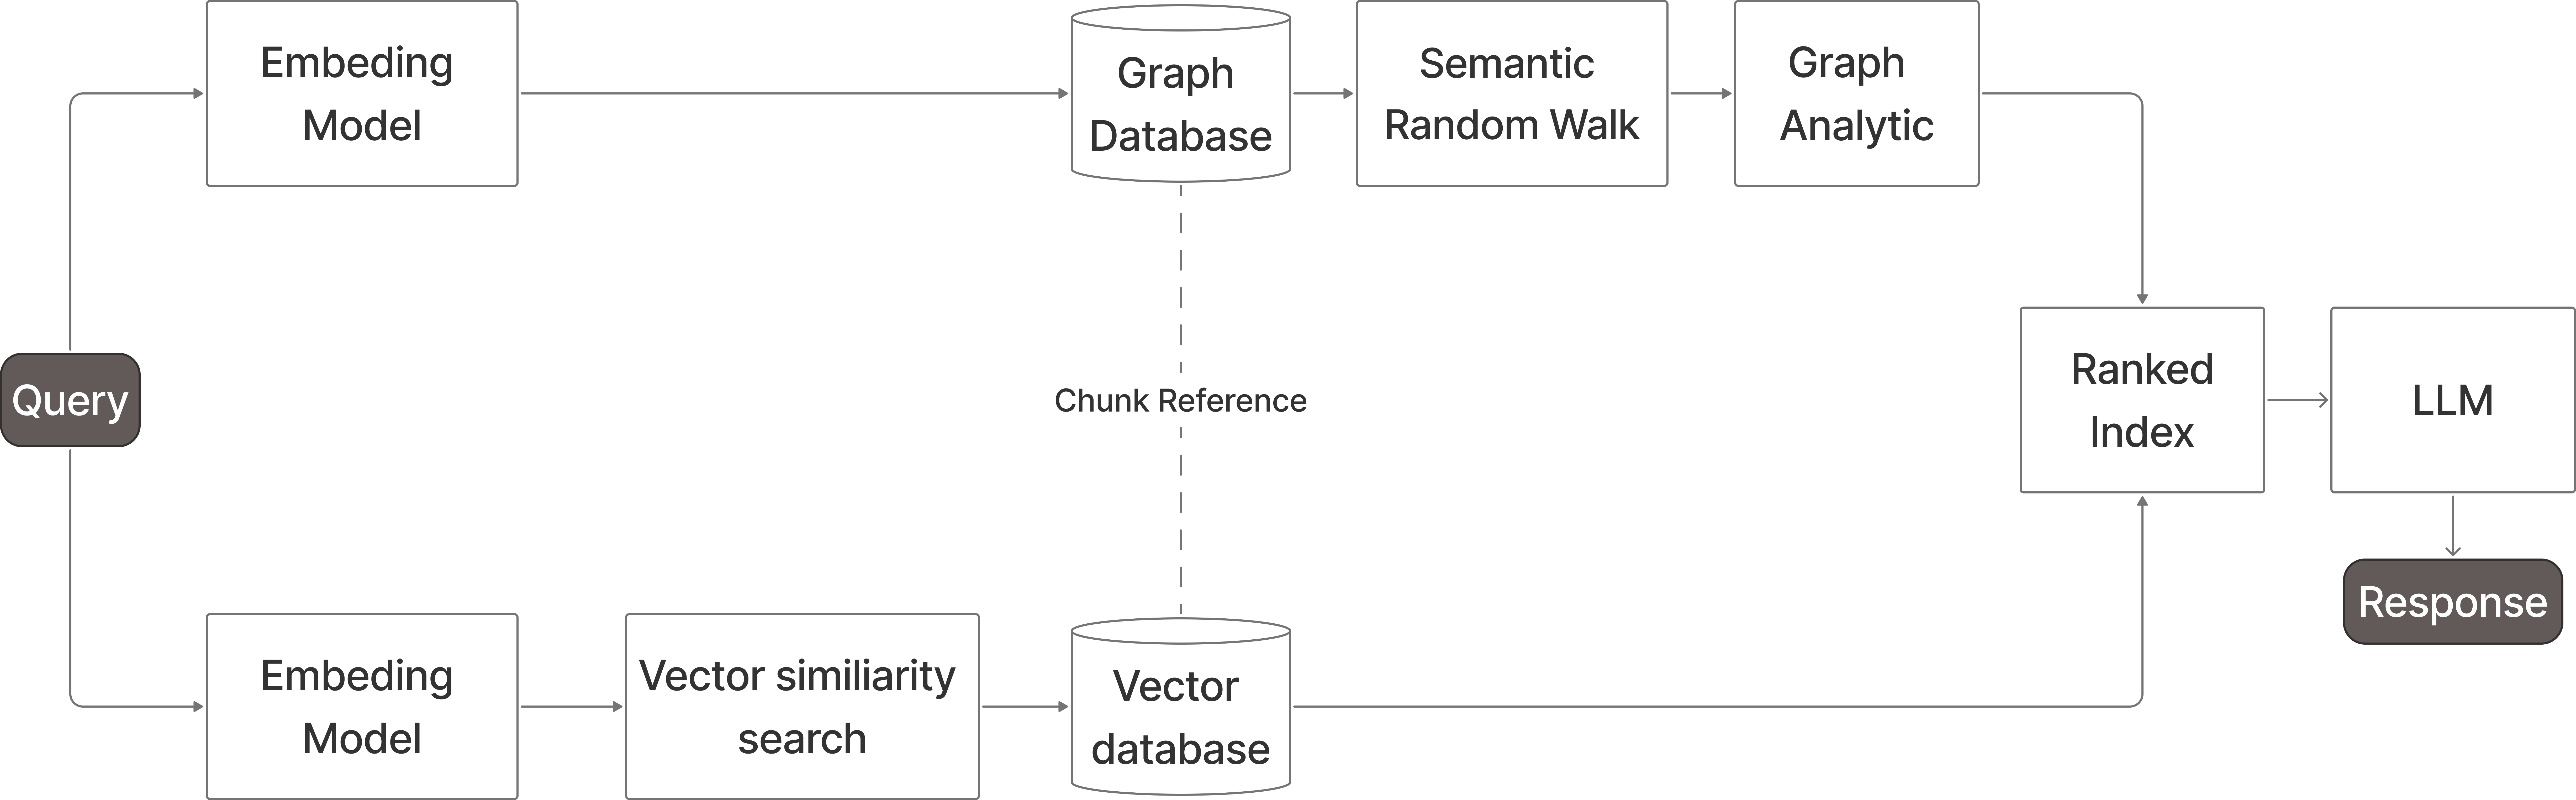
\includegraphics[width=0.95\textwidth]{Gambar/downstream app.png}
    \caption{Arsitektur pipeline konstruksi Knowledge Graph.}
    \label{fig:kg-pipeline}
\end{figure}

\textbf{Text Processing} memproses dokumen teks mentah (abstrak publikasi) yang menjadi masukan bagi pipeline. Karena keterbatasan \textit{context window} pada model bahasa, tahap ini menggunakan teknik \textit{Text Chunking} untuk memecah teks panjang menjadi segmen kalimat yang lebih kecil namun tetap utuh secara semantik, serta melakukan pembersihan karakter untuk mengoptimalkan proses inferensi.

\textbf{Named Entity Recognition (NER)} bertugas mengekstraksi entitas dari teks yang telah diproses. Penelitian ini memanfaatkan model \textbf{Gliner}, sebuah model NER berbasis Transformer yang mampu melakukan identifikasi entitas secara \textit{zero-shot}. Sistem dikonfigurasi untuk mengenali label entitas akademik spesifik seperti \textit{Task}, \textit{Method}, \textit{Metric}, dan \textit{Material} langsung dari potongan teks abstrak.

\textbf{Relationship Extraction (RE)} bertugas untuk memetakan hubungan semantik antar entitas yang telah diekstraksi. Penelitian ini menggunakan model \textbf{GliRel}, sebuah model \textit{open-source} yang dirancang berpasangan dengan Gliner untuk memprediksi relasi (seperti \textit{USED\_FOR} atau \textit{EVALUATED\_ON}) antar pasangan entitas, membentuk struktur \textit{triplet} pengetahuan.

\textbf{Graph Database} menyimpan hasil ekstraksi dari langkah RE untuk memvisualisasikan simpul (\textit{nodes}) dan sisi (\textit{edges}) sesuai dengan entitas dan tipe relasinya. Data dimuat ke dalam \textbf{Neo4j} menggunakan skema yang memastikan integritas data dan mencegah duplikasi entitas melalui mekanisme \textit{entity linking} ke node master.

\subsection{DEPENDENSI DAN KEBUTUHAN IMPLEMENTASI PIPELINE}

Berbagai alat \textit{open-source} telah digunakan untuk langkah-langkah berbeda dalam pipeline guna memenuhi kebutuhan sistem. Alat-alat tersebut dianalisis dan dipilih berdasarkan interoperabilitas, efisiensi, kinerja inferensi, dan kemudahan penggunaan. Bagian ini menjelaskan lingkungan dan pustaka yang diadopsi untuk penelitian ini.

Teknik dan alat modern digunakan untuk memastikan akurasi ekstraksi informasi pada domain akademik yang kompleks. Spesifikasi implementasi diringkas sebagai berikut:

\textbf{Spesifikasi Pipeline:}
\begin{itemize}
    \item \textbf{Text Processing:} \textit{LangChain (RecursiveCharacterTextSplitter)}
    \item \textbf{Named Entity Recognition:} \textit{Gliner (Generalist Model for NER) v2.5}
    \item \textbf{Relation Extraction:} \textit{GliRel (Zero-shot Relation Extraction)}
    \item \textbf{Graph Database:} \textit{Neo4j v5.x (Community Edition)} & \textit{Neo4j Python Driver}
\end{itemize}

\subsection{ALUR KERJA (WORKFLOW)}

Lingkungan di mana pipeline pemrosesan data dirancang dan diimplementasikan digambarkan di bawah ini. Pengaturan ini dipilih untuk mendukung komputasi model Transformer yang intensif.

\textbf{Pengaturan Lingkungan (\textit{Environment Setup}):}
\begin{itemize}
    \item \textbf{IDE:} Visual Studio Code / Jupyter Notebook
    \item \textbf{Bahasa Pemrograman:} Python 3.10
    \item \textbf{Perangkat Keras:} NVIDIA GeForce RTX 3060 (untuk akselerasi GPU)
\end{itemize}

\section{Alat Penelitian}
\label{sec:alat-penelitian}

Pengembangan sistem dan pengujian dilakukan menggunakan spesifikasi perangkat keras dan perangkat lunak sebagai berikut:

\begin{itemize}
    \item \textbf{Perangkat Keras:}
    \begin{itemize}
        \item Prosesor: Intel Core i7
        \item Memori (RAM): 16 GB
        \item Unit Pemrosesan Grafis (GPU): NVIDIA GeForce RTX 3060 (digunakan untuk akselerasi inferensi model LLM dan \textit{embedding}).
    \end{itemize}
    
    \item \textbf{Perangkat Lunak Utama:}
    \begin{itemize}
        \item \textbf{Bahasa Pemrograman:} Python 3.10.
        \item \textbf{Graph Database:} Neo4j (v5.x) untuk manajemen data graf.
        \item \textbf{Kerangka Kerja NLP:} Hugging Face Transformers, Gliner (untuk NER \textit{zero-shot}), dan GliRel (untuk \textit{Relation Extraction}).
        \item \textbf{Interface:} Streamlit untuk antarmuka pengguna \textit{Asisten Tinjauan Literatur}.
        \item \textbf{Data Processing:} Pandas untuk manipulasi CSV dan Scikit-learn untuk evaluasi metrik.
    \end{itemize}
\end{itemize}

\section{Tahapan Penelitian}
\label{sec:tahapan-penelitian}

Mengacu pada kerangka kerja yang telah dirancang, pelaksanaan penelitian dibagi menjadi tiga tahapan sistematis.

\subsection{Tahap 1: Konstruksi Knowledge Graph}
Tahap ini bertujuan mengubah data mentah CSV menjadi struktur graf. Proses ini melibatkan:
\begin{enumerate}
    \item \textbf{Normalisasi Data:} Pembersihan nama dosen, pemetaan ID unik, dan penghapusan duplikasi pada judul publikasi.
    \item \textbf{Ekstraksi Informasi (IE):}
    \begin{itemize}
        \item Menggunakan model \textbf{Gliner} untuk mengenali entitas spesifik akademik (contoh label: \texttt{Method}, \texttt{Task}, \texttt{Dataset}) dari teks abstrak.
        \item Menggunakan model \textbf{GliRel} untuk memprediksi hubungan antar entitas (contoh relasi: \texttt{USED\_FOR}, \texttt{EVALUATED\_ON}).
    \end{itemize}
    \item \textbf{Entity Linking:} Menghubungkan entitas hasil ekstraksi dengan node utama (Dosen/Proyek) yang sudah ada di basis data untuk memastikan konsistensi graf.
\end{enumerate}

\subsection{Tahap 2: Implementasi Hybrid Graph-RAG}
Pada tahap ini, dilakukan pembangunan \textit{pipeline} RAG hibrida:
\begin{enumerate}
    \item \textbf{Jalur Vektor:} Mengonversi teks abstrak menjadi vektor \textit{embedding} untuk pencarian berbasis kesamaan semantik.
    \item \textbf{Jalur Graf:} Mengonversi pertanyaan pengguna menjadi kueri Cypher untuk menarik subgraf yang relevan (misalnya: "Siapa kolaborator Dosen X?").
    \item \textbf{Generasi Jawaban:} Menggabungkan konteks dari vektor dan graf ke dalam \textit{prompt} LLM untuk menghasilkan jawaban yang alamiah dan menyertakan sitasi.
\end{enumerate}

\subsection{Tahap 3: Pengujian dan Evaluasi}
Tahap akhir meliputi evaluasi kinerja sistem menggunakan skenario pertanyaan tinjauan literatur nyata. Evaluasi diukur berdasarkan:
\begin{itemize}
    \item \textbf{Akurasi Graf:} Ketepatan ekstraksi entitas dan relasi dibandingkan dengan data manual (\textit{ground truth}).
    \item \textbf{Kualitas Jawaban:} Dinilai dari aspek relevansi, kelengkapan informasi, dan keterlacakan referensi (\textit{traceability}) terhadap sumber data asli.
\end{itemize}

\end{document}